\documentclass{article}
\usepackage{ctex}
\usepackage{graphicx}
\usepackage{amsmath}
\usepackage{indentfirst}
\usepackage{titlesec}
\usepackage{setspace}
\usepackage{subfigure}
\usepackage{caption}
\usepackage{float}
\usepackage{booktabs}
\usepackage{geometry}
\usepackage{multirow}
\geometry{left=1.2cm,right=1.2cm,top=2cm,bottom=2cm}
\title{\songti \zihao{2}\bfseries HW3第7题Data文件抽样报告}
\titleformat*{\section}{\songti\zihao{4}\bfseries}
\titleformat*{\subsection}{\songti\zihao{5}\bfseries}
\renewcommand\thesection{\arabic{section}}
\author{王启骅 PB20020580}
\begin{document}
	\maketitle
	\section{题目}
对一个实验谱数值曲线 p(x) ,自设 F(x),分别用直接抽样和舍选法
对 p(x) 抽样。比较原曲线和抽样得到的曲线以验证。讨论抽样效率。
	\section{算法原理}
	\subsection{舍选法}
观察data数据,决定取分段阶梯函数作为抽样F(x)曲线。首先将data数据归一化为概率分布数据,即每一能量点数据数除以总点数。取
\begin{equation}
	F(x)=
	\begin{cases}
		0.015& \text{,$2900\le x\le 2993 \ or \ 3005\le x \le 3013 $}\\
		0.1& \text{,$ 2993<x<3005 $}
	\end{cases}
\end{equation}


取$ \xi_1,\xi_2 $为[0,1]均匀分布的随机数列
\begin{equation}
	\xi_1=\frac{\int_{2900}^{\xi_x}F(x)dx}{\int_{2900}^{3013}F(x)dx}
\end{equation}


反解可得
\begin{equation}
	\xi_x=
	\begin{cases}
		\frac{2.715}{0.015}\xi_1+2900& \text{,$[0\ ,93/181] $}\\
		\frac{2.715\xi_1-2.595}{0.1}+2993& \text{,$(93/181\ ,173/181) $}\\
		\frac{2.715\xi_1-2.595}{0.015}+3005& \text{,$[173/181\ ,1] $}\\
	\end{cases}
\end{equation}
\begin{equation}
	\xi_y=\xi_2F(x)
\end{equation}
判断若有$ \xi_y<p(\xi_x) $则取$ x=\xi_x $。这里由于p为离散的函数,则把每一个$ \xi_x $转化为其最接近的整数点。
\subsection{直接抽样法}
取[0,1]均匀分布的随机数列$ xi_1 $,并对p(x)从2900开始挨个求和,并比较与$ \xi_1 $的大小,当求和刚好大于$ \xi_1 $时,返回上一个能量点即为所对应的$ \xi_x $。这里是由于离散点,必须通过求和的方式代替积分。
	\section{结果}
\begin{figure}[!h]
	
	\centering
	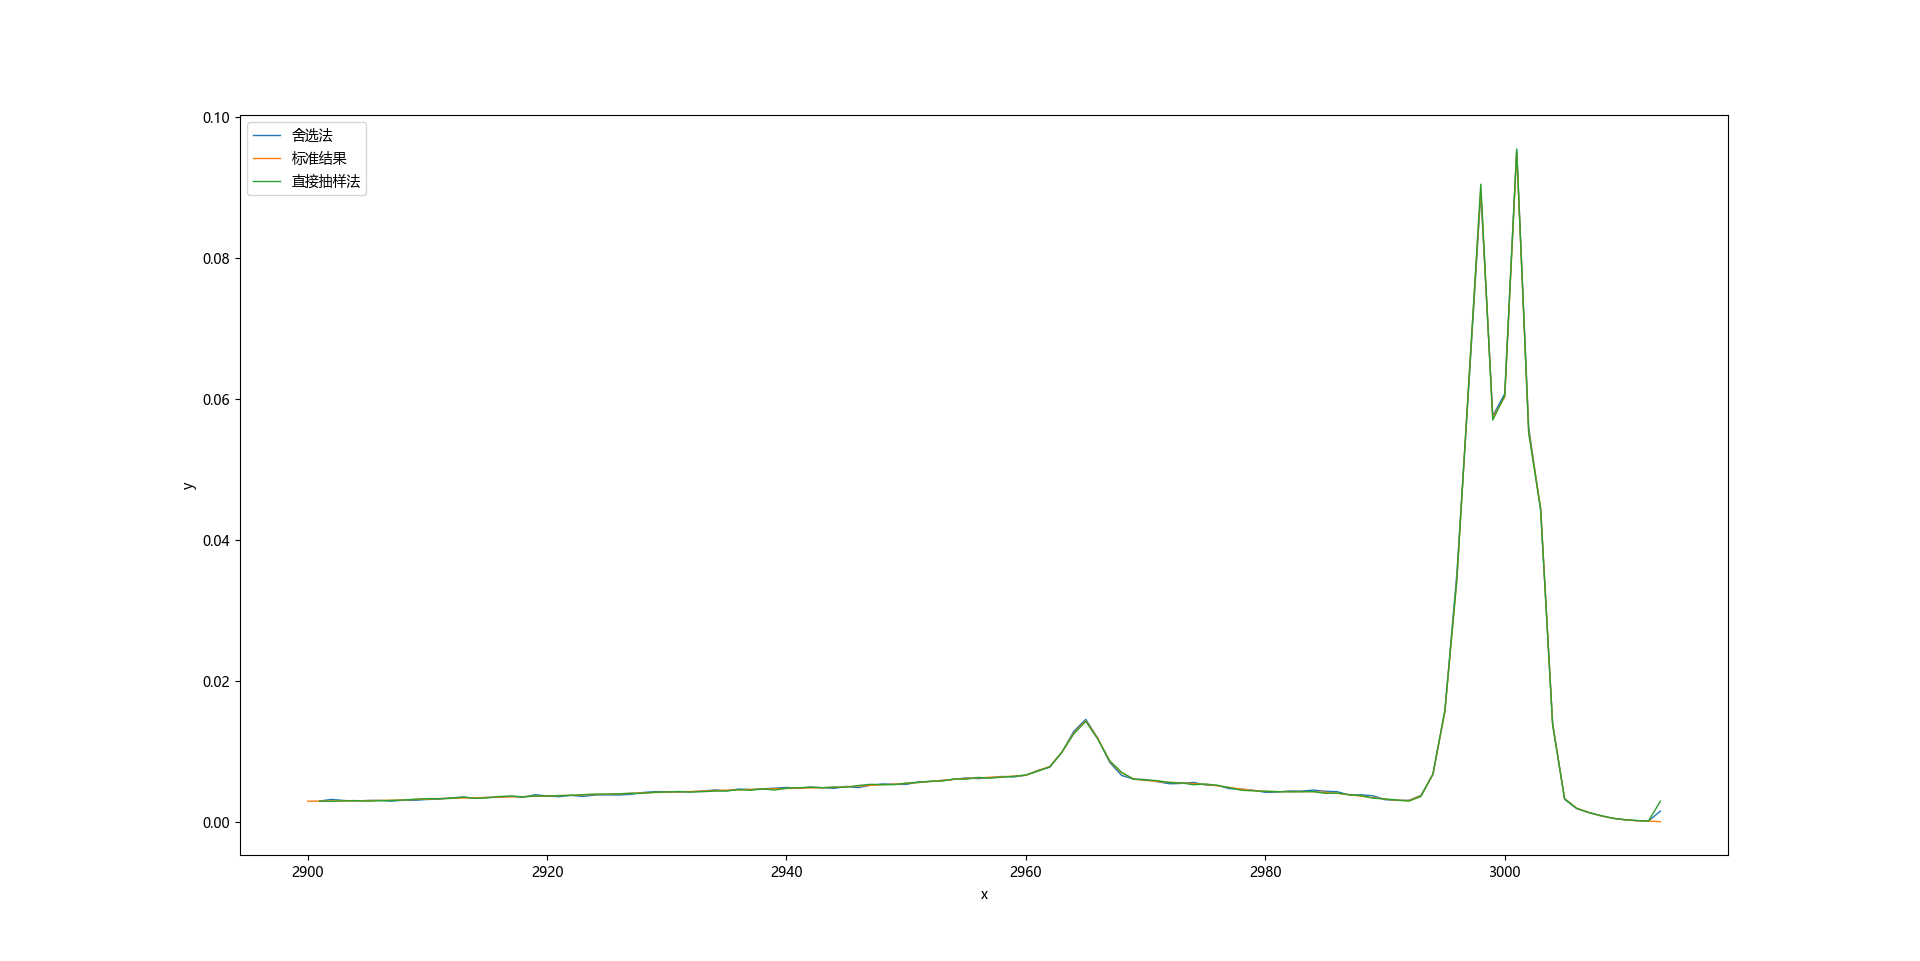
\includegraphics[scale=0.39]{data}
	\captionsetup{font={small},labelfont=bf}
	\caption{\heiti\zihao{-5}data文件抽样对比图}
	
\end{figure}
	如图1是data文件的归一化后数据图,舍选法结果与直接抽样法结果。
	
	\begin{figure}[!h]
		
		\centering
		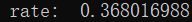
\includegraphics[scale=1]{result_3_7}
		\captionsetup{font={small},labelfont=bf}
		\caption{\heiti\zihao{-5}舍选法抽样效率}
		
	\end{figure}
如图2是舍选法抽样效率,达到0.368以上。
	\section{结论}
	可得舍选法与直接抽样法与原data数据图基本吻合。由于本身数据是离散点,所以将数据点近似到整数,用求和代替积分的方法会产生一定的误差。
	
	
	也可以通过更加细化接近原函数曲线外形的阶梯函数,分成更多区间段,来提高抽样效率。
\end{document}